%%% SVN stuff
\svnidlong
{$HeadURL: https://svn.riouxsvn.com/kneadlatxinputs/ExampleArtifactFolders/3a-SSS/SSS_Chapter_01.tex $}
{$LastChangedDate: 2024-02-23 23:39:02 -0500 (Fri, 23 Feb 2024) $}
{$LastChangedRevision: 81 $}
{$LastChangedBy: KneadProject $}
\svnid{$Id: SSS_Chapter_01.tex 81 2024-02-24 04:39:02Z KneadProject $}

\chapter{Scope}
\label{loc:Scope}
\DIDINFO{ALL-1.0 :: }


If applicable, each section has a summary of data item description (DID) information shown in this font.
These are displayed in small capital font and are not part of the formal document.
Display of these DID information notes can be turned off for formal releases, but are displayed here for reference.


This document provides the System / Subsystem Specification (\SSS) for the \ThisSystem. 
The system will be referred to as the \ThisSys.


\section{Identification}
\label{loc:Identification}
\DIDINFO{ALL-1.1 :: The \ThisSystem is an RP2040 based microcontroller board.}
This paragraph shall contain a full identification of the system to which this document applies, including, as applicable, 
identification number(s), title(s), abbreviation(s), version number(s), and release number(s).

The \ThisSystem described in this document shall be known as \ThisSys version 1.
However, the \SSS described herein shall be applicable to pre-releases such as Beta-releases for a phased release as listed for each requirement.
The major system interfaces and capabilities are fully specified in Chapter 3.


\section{System Overview}
\label{loc:SystemOverview}
\DIDINFO{ALL-1.2 :: This paragraph shall briefly state the purpose of the system to which this document applies. 
It shall describe the general nature of the system; summarize the history of system development, operation, 
and maintenance; identify the project sponsor, acquirer, user, developer, and support agencies; 
identify current and planned operating sites; and list other relevant documents. }

The \ThisSystem will be able to measure moisture levels and control irrigation in raised garden beds. 
\ThisSys is being developed by Zachary Steinberg and sponsored by University of Maryland Graduate Engineering. 
The operator and maintaner of \ThisSys will also be Zachary Steinberg. The \ThisSys will be operated outside along raised garden beds. 
\ThisSys is designed to be used by home gardeners. It is not intended for industry. \ThisSys will be controlled by a Raspberry Pi Pico W microcontroller board.

Figure~\ref{fig:SystemOverview} shows the development kit used for the \ThisSys system. 
\begin{figure}[htbp]
	\centering
		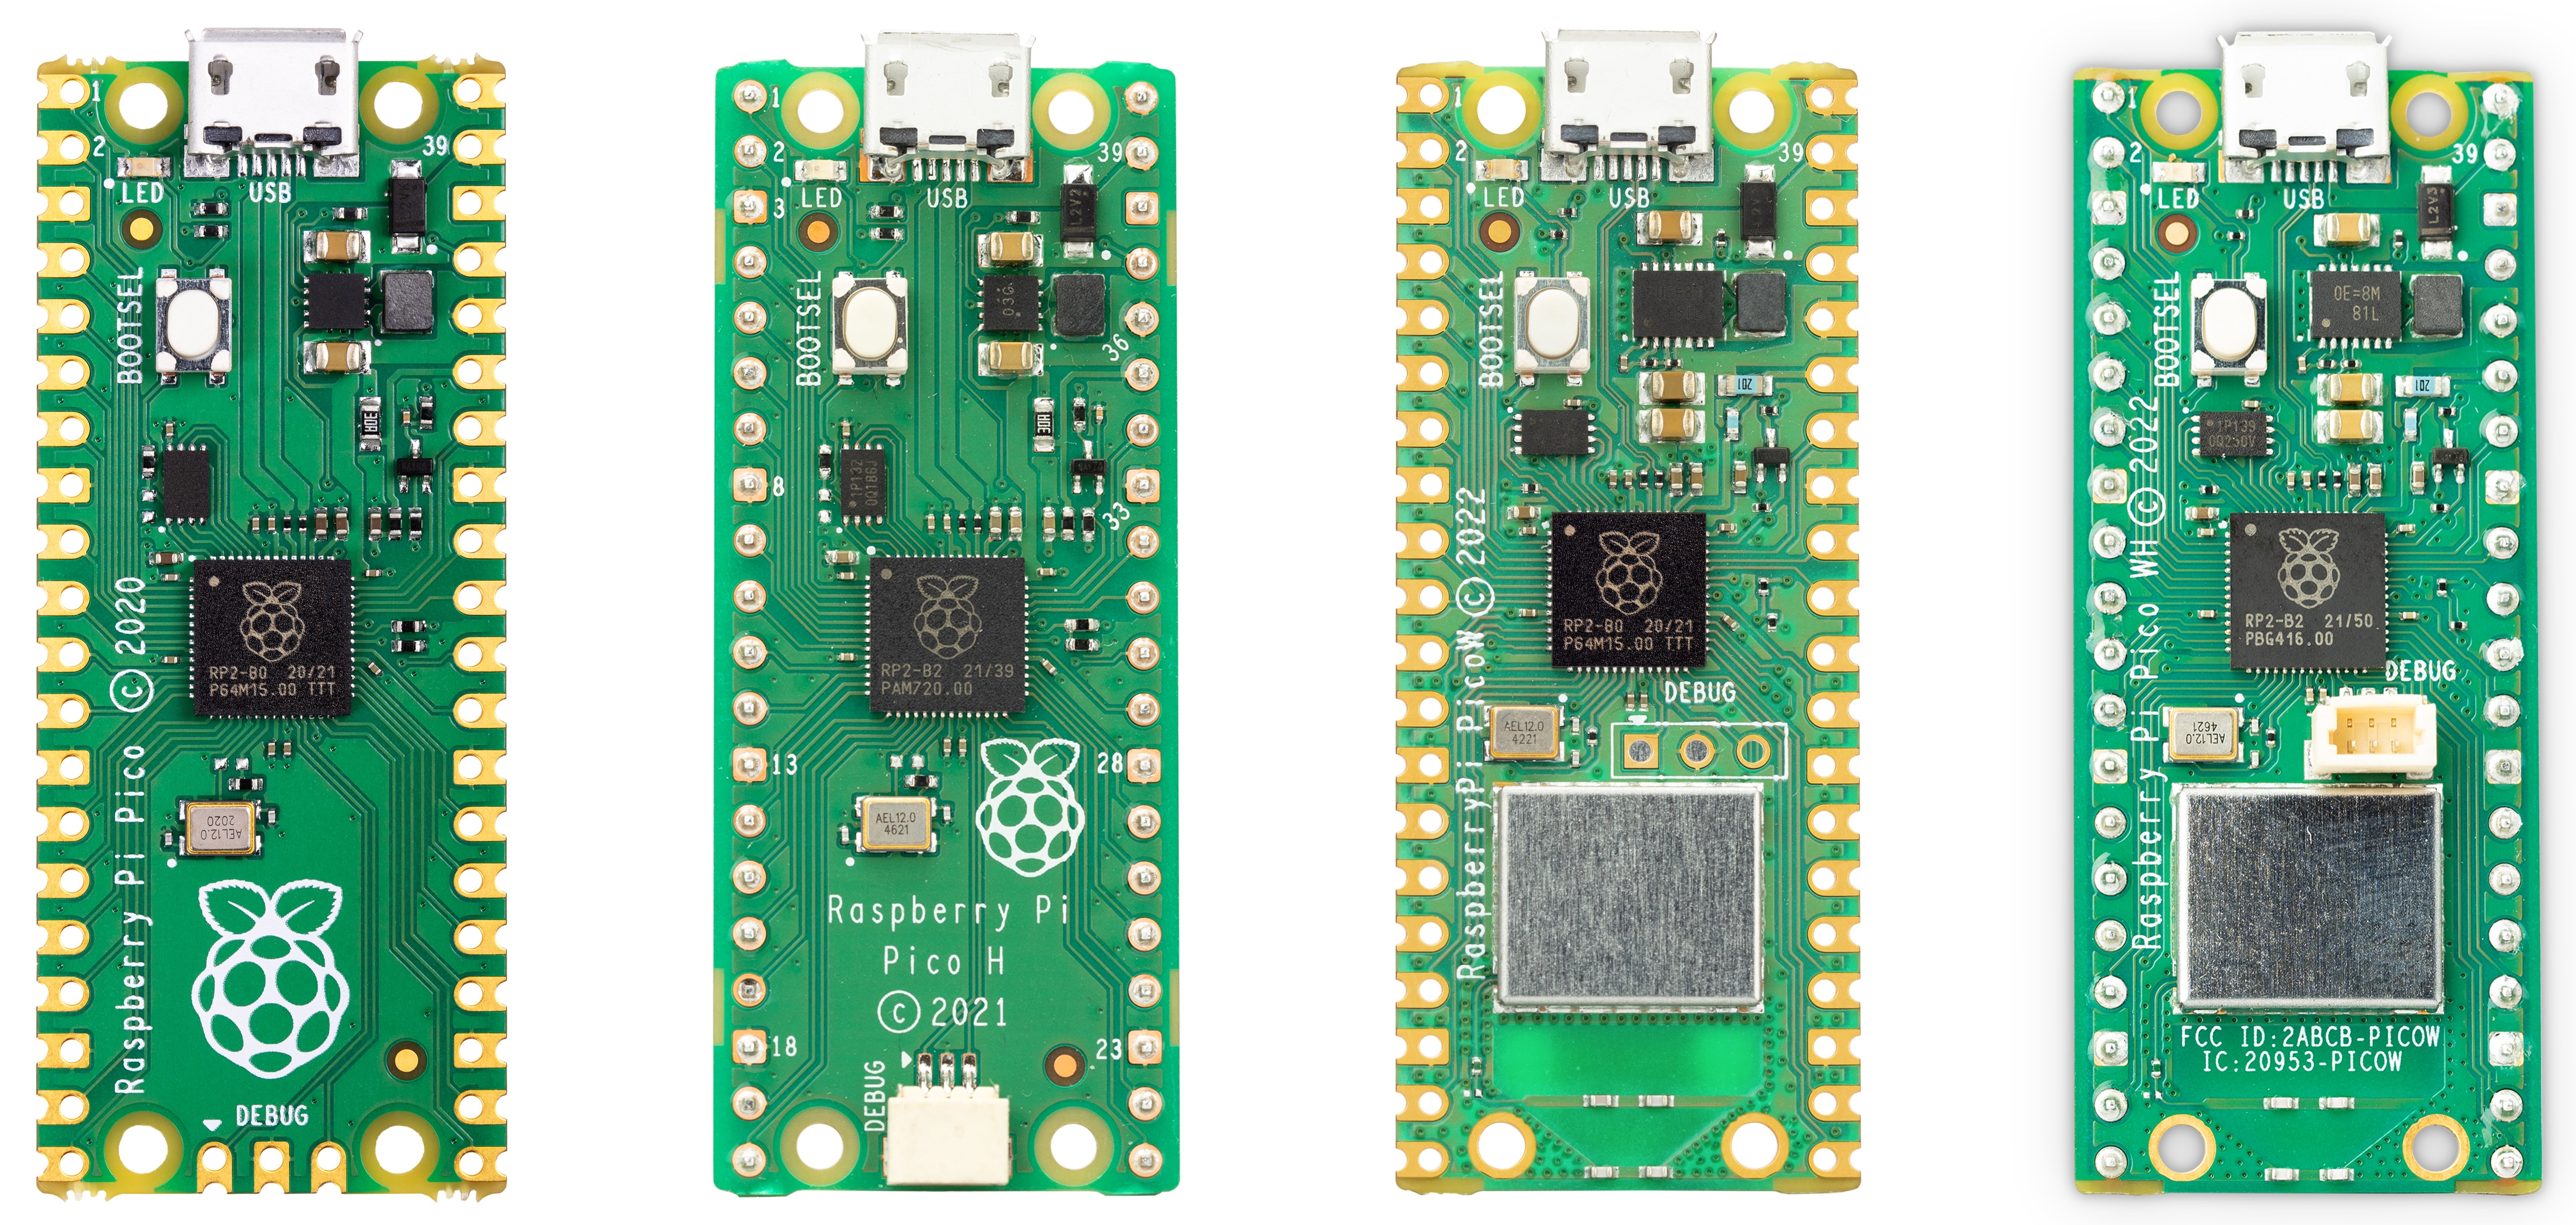
\includegraphics[width=6in]{images/pico_family.jpg}
		\caption{Raspberry Pi Pico W microcontroller board}
	\label{fig:SystemOverview}
\end{figure}
This is an image of the Raspberry Pi Pico W microcontroller board.
% This diagram shows the major external interfaces that provide the capabilities of \ThisSys.
% As are shown, the \ThisSys can provide \TBD.


% The general concept of operations (\CONOP) for this system is \TBD.








\newpage
\section{Document Overview}
\label{loc:DocumentOverview}
\DIDINFO{ALL-1.3 :: This paragraph shall summarize the purpose and contents of this
document and shall describe any security or privacy considerations associated with its use.}

This section provides information about this document's security/privacy considerations, contents, structure, and version information.
This section also provides information regarding how specifications are formatted in this artifact and how they can best be understood.

\subsection{Security and Privacy Considerations}
\label{loc:DocOverview_CUI}

%include CUI info if CUI is defined
\ifthenelse{\equal{\KNEADcuiStatus}{}}
{
	This document is not subject to \CUI restrictions.
}%endif not CUI
{% it is CUI so print CUI file info
	This document has been identified as "Controlled Unclassified Information" (\CUI).
Please follow the control block on the title page for ownership, creation, category, dissemination, and Point of Contact (\POC) information.
This information should be delineated, per \url{https://www.dodcui.mil} as:
\begin{description}[itemindent=5pt,topsep=0pt,itemsep=0pt,partopsep=0pt, parsep=0pt]
	\item[Owner] the name of the DoD Component (not required if identified in the letterhead)
	\item[Creator] identification of the office creating the document
	\item[Category] identification of the categories contained in the document
	\item[Dissemination]applicable distribution statement or limited dissemination control (LDC)
	\item[\POC]name and phone number or email of POC
\end{description}

}


This section provides information about the format of this document.
Some information provides general details about the format of this specification document.
This information, such as formatting details, is common across all levels of specification documents.
Other information is specific to this particular document.
This information is provided to assist the reader in understanding the format and layout of the information contained in this document.

\subsection{Document Sections}
\label{ssec:Intro_DocSections}

This document format is based upon the guidance in the \SRD template from MIL-HDBK-520A~\cite{ref__MIL_HDBK_520}.
The specifications and associated acceptance criteria are documented following the guidelines of ISO-12207~\cite{ref__ISO_12207} and MIL-STD-498~\cite{ref__MIL_STD_498} (from which ISO-12207 originated).
The document follows the \SSS DID~\cite{ref__SSS_DID}, with a few minor tailoring changes.


The first format tailoring change allows for the system interfaces to be specified before the system capabilities. 
This follows standard structured design practice (e.g. Yourdon's Structured Method) whereby the system context is provided before the design itself.
The net result of this change is that system capabilities are presented in section 3.3 instead of 3.2, as prescribed in the \SSS template, and external system interfaces are described in section 3.2 instead of section 3.3 as prescribed in the \SSS template.
This allows the data inputs to the system to be defined {\em before} they are used in the capabilities section.

The second format tailoring change relates to placement of general material within the document. 
The qualification provisions and traceability details, if applicable, are listed with each requirement.
This formatting, which is allowed in the \SSS DID~\cite{ref__SSS_DID}, allows the reader to view all relevant information for each requirement in a single location, rather than requiring constant page turning.
This information may be duplicated in Sections 4 and 5, respectively, but if done this way, it can be generated automatically to prevent manual duplication errors.
The table of acronyms is also listed in chapter two, versus the notes section, so that it may be parsed by readers before encountering most of the acronyms.

Otherwise, this document follows the listed \SSS sub-section order.
\begin{description}
	\item[Section 1] provides an overview of the system and this document.
	\item[Section 2] lists general and application-specific reference documents as well as glossary terms and acronyms. 
	\item[Section 3] details the specifications for the system.
                    %See section~\ref{ssec:Intro_SpecFormatting} for more information regarding the traceability issues.
	\item[Section 4] maps the specifications to quality provisions. 
                    %See section~\ref{ssec:Intro_SpecTrace} for more information regarding the traceability issues.
	\item[Section 5] traces specifications to the original source.
                    %See section~\ref{ssec:Intro_SpecTrace} for more information regarding the traceability issues.
	\item[Section 6] if needed, lists any general notes as may be applicable beyond any notes provided in the requirement and expectation tables in section 3.
	\item[Appendices] if needed, provide additional information as may be needed.
\end{description}

\subsection{Document Version Information}
\label{loc:DocOverview_LaTeXAndSvnVersionInformation}

This document was produced in \LaTeXx and \Biberx.
The editing and document preparation were performed using MiK\TeX{} version 2.9  with the build option $[$\LaTeX{}  $\Rightarrow$ PS $\Rightarrow$ PDF$]$.
The \LaTeXx {\em svn-multi} package was used to glean SVN tracking information, when files are stored in an ``SVN'' version control system.
The style {\tt \KNEADdocumentClsName}
%, which was based on the style provided in~\cite{ref__thesisguide}, 
was used to provide the \LaTeXx and \Biberx formatting details.

% This revision of this document has the following properties:
% \begin{table}[htbp]
	% \caption{Subversion (SVN) Data}
	% \label{tab:SVNdata}
	\centering
		\begin{tabular}{|p{1.5in}|p{4.9in}|}
		%%%%%S\multicolumn{2}{c}{\bfseries SVN Information} \\
		\hline
			{\bfseries Tracking Item}  &  {\bfseries Data} \\
		\hline		
		\hline
			Repository         & \url{\svnmainurl}  \\
		\hline
			Author         & \svnauthor  \\			
		\hline
			Revision       & \svnrev     \\	
		\hline
			Rev Date       & \svndate    \\	
		\hline	
			Print Date     & \today{} \currenttime    \\	
		\hline
			\KNEADdocumentClsName\break Version     & \KNEADdocumentClsVersion    \\	
		\hline	
			\KNEADdocumentClsName\break Date        & \KNEADdocumentClsDate   \\	
		\hline
		%%%\DocumentTexName\break Version     & \DocumentTexVersion    \\	
		%%%\hline	
		%%%\DocumentTexName\break Date        & \DocumentTexDate   \\	
		\hline						
    \end{tabular}
\end{table}

\subsection{Specification Formatting}
\label{ssec:Intro_SpecFormatting}

The specifications are listed and numbered by document sections. 
The fully qualified specification numbers include the sub-section in which it is contained. 
These specification numbers are tied to the document level thus they are numbered from 1 to N for each sub-section of the requirements section. 
This is done to allow for additions within a sub-system without affecting the numbering in other sub-systems. 
Once a specification has been added, it cannot be deleted, only its status may be changed to ``inactive'' or ``deleted'' to preserve numbering.

This document allows for marking changes to specifications.
All specifications may be marked with a change bar.
This generally implies that one or more parts of a specification changed from the prior revision.
A note should be provided to indicate the reason for the change, and when, so that future versions of the document, which do not include the change bar, still have rationale included for the current value.

%The table format also allows for grouping of related specifications.
%These grouped specification are also numbered sequentially and are also not removed if made inactive. 
%Rather, they are marked in a ``strike-though'' font to denote that they are inactive or deleted.

The system specifications are listed in a common table format as shown in Requirement~\ref{rqt:TableFormat}.
%%% \ONERQTM[8] is macro for consistently formatted requirements
\ONERQMT
% #1 is the requirement number
{1.3.1}
% #2 is title
{Specification Table Format}
% #3 is requirement label (expected to be of form rqt:XXX)
{rqt:TableFormat}
% #4 is the requirement text
{
\begin{my_enumerate}
	%1,2,3
	\item The first row of a table provides a unique number and a title for the requirement or expectation. This row is generated from the first 3 arguments.

	%4
	\item The second row of the table provides the specification text of the requirement. Normally this is a single sentence with a single testable requirement (shall) statement. This example uses an enumerated list in order to describe all the rows in a single table.

	%5
	\item The next row of the table provides the status for the specification listed in the table. This includes the applicable phases or release versions in which the required feature is supported, where S $\in$ \{(T)hreshold, (O)bjective, (I)nactive, (D)eleted\}.
  
	%6
	\item The next row of the table provides the acceptance criteria. This row follows the form of ``This requirement shall be verified by V $\in$ \{inspection, demonstration, test, analysis\}.'' Additional information regarding testing can be provided in the notes section.

	%7
	\item The next row of the table provides the traceability of the requirement. The traceability connects the requirement to a higher level document that calls out the need for a requirement. The structure of traceability is expected to be of the form ``This requirement traces to MIL-STD-498~\cite{ref__MIL_STD_498} and ISO-12207~\cite{ref__ISO_12207}.'' Note that the source is expected to be listed in the reference documents section.

	%8
	\item The final row of the table provides, if applicable, notes for the specification. Notes are not a formal part of the requirement or expectation but provide supporting information regarding the feature.
 \end{my_enumerate}
}
% #5 is status (active, inactive, etc.)
{
	\item [All phases] This format is active for all specifications in this document.
}
% #6 is Acceptance
{This specification is not a testable requirement for the system; it is for demonstration purposes only.}
% #7 is traceability
{
	\item [N/A] There is no traceability for this requirement.
}
% #8 is notes
{
   \item This table is generated using a \LaTeX{} command.
   \item This formatting is not a testable requirement on the system, but rather, shows how each requirement is depicted in this document.
}
% #9 is last version in which this specification was changed, to create a changebar.
{P1}
%%%%% end \ONERQTM[9] macro

The status designations for each specification S $\in$ \{(T)hreshold, (O)bjective, (I)nactive, (D)eleted\} are based on the following criteria.
\begin{my_description}
{
\item [\OneRqmtThreshold] Items marked ``\OneRqmtThreshold'' are driven by the project threshold needs that must be met in the specified phase.

\item [\OneRqmtObjective] Items marked ``\OneRqmtObjective'' are objective goals of the system in the specified phase. These requirements may stay (O) for all listed phases or may transition from (O) to (T) in future phases. This provides hints as to future expansion of system capabilities so the design can account for the feature without significant later rework.

\item [\OneRqmtInactive] Items marked ``\OneRqmtInactive'' are requirements that are not currently to be met by the system in the specified phase. Unlike `\OneRqmtObjective'' requirements, (I) requirements may be in limbo in terms of certain details but their inclusion may also provide hints as to future expansion of system capabilities. 

\item [\OneRqmtDeleted] Requirements that are not to be met by the system are marked by ``\OneRqmtDeleted''. Use of this status, vice removal of the requirement text, preserves the numbering of subsequent requirements and notes that the requirement once was invoked.
The rationale for the deletion should be included in the notes section. 
}
\end{my_description}

External tools have been written that allow for automatic generation of other documentation.
Specially, data for chapters and appendices that follow the requirement specifications, can be gleaned automatically to ensure integrity between the sections of the documents.
In addition, the listing of \KPP and \KSA values into a ``B-spec'' can be automated.
Finally, the full set of requirements, and the associated attributes, are exported to a comprehensive \CSV file for import into external tools such as \DOORS.


This table approach offers other advantages besides automated parsing for import into tools.
As can be seen in Table~\ref{rqt:TableFormat}, and in all the specifications, this format groups all information for each specification into a separable and easily viewed structure.
The document sections and subsections provide a logical grouping of the specifications but the table allows all pertinent information to be grouped, vice being split across major sections of the document.
This grouping allows for easier presentation since each grouping is similar to a ``PowerPoint'' presentation slide.
And, as will be seen in Section~\ref{ssec:Intro_HowToRead}, it can help the writer organize specifications.
The approach also allows for a ``List of Specifications'' to be generated.
Each table is listed in the list of specifications so that each high level grouping can be quickly located from the list.
Of course, the tables are located in the appropriate sections as noted in Section~\ref{ssec:Intro_DocSections} so they can be found in that manner as well.


Another major advantage of the table format is the ``Notes'' section.
As specifications are developed, there will be many issues to be resolved.
And, once issues are clarified, tracking the rationale for the decision is just as important as recording the answer~\cite{ref__Brooks_MMM}.
Thus the notes section helps the reader and the writer.
The writer has a logically grouped place to put notes for each specification and the reader can easily find them without having to refer to footnotes, separated sections, or external documentation.



\subsection{How To Read Specifications}
\label{ssec:Intro_HowToRead}

System Performance Specification (\SPS) documents, by their very nature, are a collection of independent but interconnected facts.
Systems require interfaces from which inputs are consumed and to which outputs are produced.
These input data are transformed by the capabilities to produce the outputs.
The entire system has myriad other requirements ranging from data formatting through physical limits on things like the enclosure and packaging.
Finally, at the system level, specifications need to dictate {\em what, and, how well} a system must perform.
Likewise, in order to separate documentation functionality, the \SPS should not state explicitly {\em how} the system is to be formed, except in very special circumstances.
Given the disparate nature of the requirements, system performance specifications can be hard to digest.


System / sub-system Segmentation Specification (\SSS) and Software Requirements Specification (\SRS) documents suffer from many of the same issues as do \SPS documents.
An \SSS turns the performance specification into a first level design.
Where the \SPS has disparate performance requirements, the \SSS has disjoint hardware and software configuration items listed as well as a mapping of the two items on to, and in to, each other.
For the requirement management function, each element of the system design in the \SSS traces back to the overall \SPS specifications.
Only at the \SRS level do the requirements start to focus on a single item.
Thus, the \SSS and \SRS level documents describe share a common contextual issue with the \SPS document.


An understanding of the documents' structures is needed to help parse the information.
The developers of MIL-STD-498~\cite{ref__MIL_STD_498}, however, understood this and devised a format that can help manage the information overload.
The method by which this is accomplished is to organize requirements into eighteen specific groupings.
By understanding these groupings, a reader can improve their understanding of the system described by the requirements by understanding that specific information is listed in specified sections.


These documents follow a {\em read-forward} mentality so that base information is provided before it is actually needed.\footnote{In fact, the read-forward philosophy extends across the documents as well but that topic is beyond the scope of this discussion.}
For example, the referenced documents (and in this document the list of acronyms and glossary terms) are provided in the second chapter, before most items are actually cited.
By presenting this information to the reader before citation, the format allows the reader to glean upfront information about the kind of things that will be covered later on in the document.
Presentation of the referenced material ahead of the document body also allows the reader to have a priori information before encountering the symbol in the text.
By understanding these formatting clues, the reader is able to be prepared for what is coming further down the road in the document.


Another reason for this organization is that different readers process information differently.
There is no one format that will be best for all readers.
By having the information in standardized sections across all such performance specifications, however, readers can use the document as a reference as needed.
As an example, Section 3.1 of these documents will always define the system states and modes.
If a reader wants to look up this information, it is always in that section.
And, since it is listed first, all ensuing sections can reference states and modes in order to qualify their requirements.
Likewise, having external interfaces presented {\em before} the capabilities means that the capabilities can define the transformations without having to worry about how the data is ingested into the system; the data is already ``in the system'' from a reader's point of view when the data is needed to define the transformation.


This separation between, and the presentation order of, the data and processing is important when the same data supports multiple capabilities.
A hierarchical description of ``derived'' requirements often would have a capability definition leading to the requirements for the data needed by the capability.
In the case, which occurs often, where the data is used in two different transformation capabilities, a hierarchical approach of capability leading to external interfaces is met with the problem of which capability gets to have the data interface in its tree.
This approach also leads to the dilemma of what to do when that first capability is no longer needed by the system but the second capability, and thus the data defined under the first capability tree, still {\em is} needed by the system.
Just as loosely coupled software is more maintainable, so are loosely coupled requirements.


A final note about reading actually comes from ideas about how to write a requirement document.
The document format dictates a linear flow from start to finish.
A reader often reads a document the first time from front to back; this is why the {\em read-forward} approach works.

The writer, however, is {\em not} constrained in the same linear manner.
Thus, while writing requirements about a capability, the idea for a new state or mode may arise.
The writer can easily jump to the states and modes section in order to add in the information and then return to complete the capability that led to the new state or mode, safe in his knowledge that when the reader sees this new specification, they should have already seen the newly defined state or mode that is used to qualify the requirement since the state or mode was already presented in an earlier section.

Readers can use this information to enjoy the fact that the writer jumped around in the writing phase to save the reader the same effort when trying to read the document.
By understanding the sections and the expected contents of the sections, which are defined in the \SSS DID~\cite{ref__SSS_DID} and the related MIL-STD-498~\cite{ref__MIL_STD_498} document templates, a reader can read cover-to-cover, or jump to the needed information quickly, knowing that the writer put the information in the specified sections to make finding the information easier for the reader.

\subsection{Specification Traceability}
\label{ssec:Intro_SpecTrace}% must be labeled this since it is referenced above

A project typically has several levels of statements of what needs to be done.
Often an Operational Concept Description (\OCD) is developed to provide a high level description of the system to be developed and its expected uses.
A set of documents that follows the MIL-STD-498~\cite{ref__MIL_STD_498} \DID formats is often developed for a project.
A Statement of Work (\SOW) or a Statement of Objectives (\SOO) is often developed to direct contractors on a project.
While a \SOW or \SOO is supposed to be more contractual statements of tasks and objectives rather than actually trying to specify what needs to be built, these documents often, however, do include system requirements.
A better method is to have the \SOW or \SOO reference a formal \SPS so that the full scope of the system can be defined.
Situations for every project differ so the main thing to understand is that there will be many documents and that their contents need to be related to each other.


Given the number of specifications for a system, and all the levels at which the specifications may be written, understanding if all needs of a system are being met is critical.
Different documents have different levels of specifications and design materials.
A mapping between the specifications at all of the different levels is essential to make sure that the design meets all of the stated needs of the system and that the system does not include capabilities that are not required.


As a system performance specification, the \SPS is the highest level of specification of systems requirements.
This document defines {\em what} the system needs to do without saying {\em how}.
Thus, in general, there should be nothing higher to which the requirements in a \SPS can be traced.
In practice, however, some document such as an \OCD for the system, informal customer requirements documents, or a \SOW or \SOO for the project may be provided that indicates some of the system needs.
If the specifications in the \SPS meet all the use cases in the \OCD then the system meets the needs but only if the use cases are all inclusive.
Likewise, if the \SOW or \SOO tries to list things the system needs to do, these needs must be tracked.
And, of course, statements of need in any straw-man requirements documents need to be met.
Once the fully developed \SPS specifications are captured then the higher level document(s) be examined to make sure that, at a minimum, all of those things listed are captured in the \SPS.
This process ensures that the \SPS is compliant with the other ``defining'' stakeholder documents.


To ensure coverage compliance, each of the higher level needs, whether implied or explicitly stated, needs to be mapped to the \SPS specification(s) that cover each given need.
This is expected to result in a one-to-many relationship where many of the \SPS specifications are mapped to a single upper level need.
And, each specification in the \SPS can be mapped to multiple needs depending on the independence of the needs.
The details of how to do this mapping, which is best handled through some relational database tool (e.g. \DOORS), are beyond the scope of this introduction.
The important thing to note is that this traceability determines if the \SPS covers the known needs of the system.
Since a well-formed \SPS includes many more facets than an \OCD or \SOW / \SOO, there may be orphan \SPS requirements that do not map directly to the higher level documents.
However, there can be no orphan needs from the stakeholder documents that do not map to the \SPS.
The key here is to perform a mapping between the \SPS and any higher level stakeholder documents to ensure that the specifications of the \SPS provide compliance to the higher document(s).


Another way of saying this is to summarize the overall design philosophy as follows: a level of design should be carried out and mapped to higher level artifacts rather than simply ``deriving'' requirements from the higher level documents.
This mapping process, thus, is {\em not} a way to derive a fully defining set of requirements for the \SPS.
The act of ``deriving'' specifications of system from a non-specification document such as a \OCD, \SOW, or \SOO does {\em not} ensure that all the true system needs are captured.
In fact if this approach is followed then often many requirements are missed because of the incomplete nature of the \OCD, \SOW, or \SOO list of system needs.


An \SPS, just like any level document, needs to be developed using domain knowledge and by following best practices and a well-defined documentation format.
All of the things that must be considered for defining a successful system need to be included in the \SPS.
Note that, obviously, if the \SOW did all of this then the \SOW would be the \SPS.
But, in practice, this rarely ever happens, nor should it.
The \SOW or \SOO are programmatic level documents that list things to do to build the system; they are not supposed to define the system.
This is the job of the \SPS.


The system / sub-system segmentation specification (\SSS) is the second level of specification of systems requirements.
The \SSS starts to define {\em how} the system will meet the needs and should include a top-level system decomposition (or segmentation) of capabilities from the \SPS to the sub-systems of the system.
In a typical documentation set, there should be a higher-level document (i.e. the \SPS) to which the specifications in the \SSS can be traced.
The goal here is to ensure compliance with the higher level document much as was done with the \SPS and higher level programmatic documents.
If the design specifications in the \SSS cover all the performance specifications in the \SPS then the system design covers the documented system needs.
This does not mean that the system {\em will} meet the performance specifications, it just means that there are no obvious holes.
And, of course, if some \SPS specifications are not covered in the \SSS then those specifications obviously cannot be met by the system design.


Since the \SPS and \SSS documents are all explicit statements of requirements, there can be no gaps between the specifications in them.
If there is no mapping from at least one \SSS requirement to each of the \SPS requirements then the system cannot meet the stated requirements of the \SPS.
While the goal here is to ensure that the specifications of the \SSS provide coverage to the higher document, true compliance can only be determined through design analysis and testing efforts.
And, if there is an orphan \SSS requirement then the questions must be asked: ``Why is this requirement included?'' and ``Can this requirement be deleted?''.
Taken together, the \SPS and \SSS documents can form the basis for a well-formed design artifact set: 
References to higher-level artifacts document where the system goals came from and the code (and hardware) level artifacts (source code and CAD models) should describe the final product details. 
Coupled with appropriate test documents, this level of design process and documentation generation should adequately allow for successful development while preserving the architectural aspects for future revisions and modifications.



{\em 
Because this is the overall system performance specification, this document may provide traceability to miscellaneous project documents.
This allows for tracking of related doctrine, vendor, and draft specification requirements as the document is being created.
}



